\documentclass[twocolumn]{article}

\usepackage[english]{babel}
\usepackage[a4paper, top=2cm, bottom=2cm, left=3cm, right=3cm, marginparwidth=1.75cm]{geometry}
\usepackage{graphicx}
\usepackage{hyperref}

\title{Alternative Splicing}
\author{Anamaria Hodivoianu, Class 332}

\begin{document}
\maketitle

\section{Introduction}
Alternative splicing is a process in which a single gene can generate multiple proteins. This works because the exons, the parts of the gene that encode the information needed for the protein, can be spliced in different ways. This is important because it means that even with a relatively small number of genes, a large number of proteins can be created.

\begin{figure*}
    \centering
    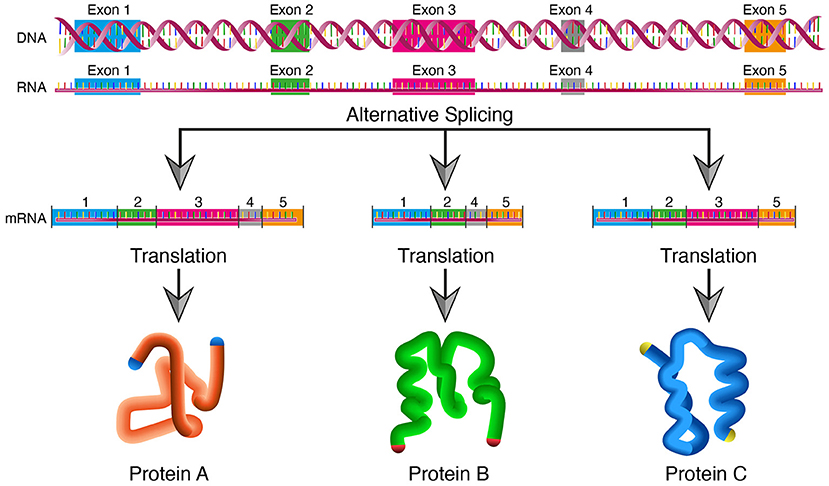
\includegraphics[width=0.8\textwidth]{figure-3.jpg}
    \caption{Alternative splicing generating different proteins. Source: \url{https://www.frontiersin.org/files/Articles/1063940/frym-11-1063940-HTML-r2/image_m/figure-3.jpg}}
\end{figure*}

\section{Discovery}
Alternative splicing was discovered in 1977 in the adenovirus. Researchers observed that the virus generates five primary RNA transcripts before the DNA replication, and another, much larger one after. The scientists found that the last transcript was spliced in different ways, which generated different proteins. 
Alternative splicing was first observed in mammals in 1981, in the gene that encodes calcitonin, the thyroid hormone.The gene contains 6 exons, but the calcitonin mRNA contains only the first four. This gene was found to also generate another mRNA, which contains all the exons except the fourth one. This generates the calcitonin gene related peptide (CGRP).
These are examples of biologically relevant alternative splicing, but there are many more which have been discovered. Currently, it is estimated that 95\% of human genes undergo alternative splicing. The gene that has the most alternative splicing variants is D. melanogaster, or the Dscam gene, which has 38.016 possible splicing variants.

\section{Splicing Modes}
There are several modes of alternative splicing. The following five are the basic, generally recongnized ones:
\begin{itemize}
    \item Exon skipping / cassette exon: An exon is excluded from the final mRNA. This is the most common one in mammals.
    \item Mutually exclusive exons: Only one of two exons is included in the final mRNA.
    \item Alternative 5' donor site: the 5' end of an exon is spliced to different sites.
    \item Alternative 3' donor site: the 3' end of an exon is spliced to different sites.
    \item Intron retention: an intron is included in the final mRNA. This is the least common one in mammals.
\end{itemize}
These modes can appear in different combinations, leading to a large number of possible proteins.

\begin{figure}
    \centering
    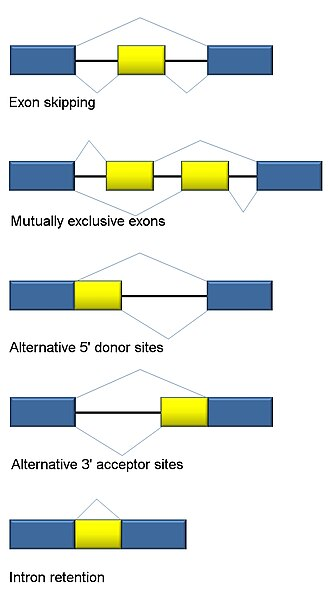
\includegraphics[width=0.5\columnwidth]{Alt_splicing_bestiary2.jpg}
    \caption{Alternative splicing modes. Source: \url{https://upload.wikimedia.org/wikipedia/commons/thumb/a/ab/Alt_splicing_bestiary2.jpg/220px-Alt_splicing_bestiary2.jpg}}
\end{figure}

\section{Importance}
Alternative splicing is very useful for humans and other organism because it allows for a large number of different proteins to be created from a smaller number of genes. Although the human genome contains only about 20.000 genes, humans can produce between 80.000 and 400.000 proteins which have different functions. There has been some research that compares the number of genes in humans and in other organisms, such as the roundworm C. elegans, and the fruit fly D. melanogaster. It was found that the number of genes in humans is by 30\% bigger than in the roundworm, and twice as big as in the fly. This shows that alternative splicing is very important for the complexity of the human body. Another study compared the frequency of alternative splicing in humans, mouses, rats, cows, the fruit fly, and the roundworm. It took 100.000 expressed sequence tags (EST) from each organism, and it found no major difference between the frequencies of alternative splicing. However, a later study compared the frequencies by randomly selecting subsets of genes, and found that vertebrates have a higher frequency of alternative splicing than invertebrates.

\section{Conclusion}
In conclusion, alternative splicing is a process that selects different exons from a single gene to generate different proteins. This is very important for the complexity of the human body, as it allows for a large number of proteins to be generated from a smaller number of genes.

\section{Bibliography}
\begin{thebibliography}{99}
    \bibitem{1} Wikipedia. \textit{Alternative splicing}. Link: \url{https://en.wikipedia.org/wiki/Alternative_splicing}
    \bibitem{2} National Human Genome Research Institute. \textit{Alternative splicing}. Link: \url{https://www.genome.gov/genetics-glossary/Alternative-Splicing}
    \bibitem{3} National Center for Biotechnology Information. \textit{Mechanism of alternative splicing and its regulation}. Link: \url{https://pmc.ncbi.nlm.nih.gov/articles/PMC4360811/}
    \bibitem{4} The Scientist. \textit{All About Alternative Splicing}. Link: \url{https://www.the-scientist.com/all-about-alternative-splicing-72189}
    \bibitem{5} Baylor College of Medicine. \textit{Alternative Splicing}. Link: \url{https://www.bcm.edu/research/faculty-labs/tom-cooper-lab/alternative-splicing}
\end{thebibliography}

\end{document}